%\newcommand{\View}{
%  \href{https://developer.android.com/reference/android/view/View.html}{View}
%}

%\newcommand{\ViewGroup}{
%  \href{https://developer.android.com/reference/android/view/ViewGroup.html}{ViewGroup}
%}

\newcommand{\AdapterView}{
  \href{https://developer.android.com/reference/android/widget/AdapterView.html}{AdapterView}
}

\newcommand{\Adapter}{
  \href{https://developer.android.com/reference/android/widget/Adapter.html}{Adapter}
}

\Section{Макеты (Layouts)}

\Subsection{Макет}

Макет (англ. Layout) определяет то, как будет выглядеть структура UI. Создать
layout можно двумя способами:
\begin{itemize}
  \item \textbf{Описать элементы UI в XML-файле.} Андроид предоставляет
  прямолинейный XML синтаксис, который соответствует классам и подклассам
  \View.
  
  \item \textbf{Создать элементы layout во время выполнения.} Приложение может
  создавать объекты \View и \ViewGroup (и изменять их свойства) программно. 
\end{itemize}

Фреймворк Андроида позволяет гибко использовать только один или сразу оба из
этих способов, для создания и управления UI приложения.
Преимуществом создания UI в XML является тот факт, что внешний вид приложения
отделяется от кода, который управляет логикой.

\Subsection{Стандартные макеты}

Каждый подкласс класса \ViewGroup предоставляет уникальный способ для
отображения \View, которые он содержит внутри.

\textbf{Замечание:} Хотя и можно помещать один layout в другой, чтобы добиться
желаемого внешнего вида, не стоит этим злоупотреблять. Следует стараться
сделать иерархию как можно меньше. Layout рисуется быстрее, если у него мало
вложенных layout (широкая иерархия лучше, чем глубокая).

Вот некоторые наиболее часто используемые виды layout, которые предоставляются
платформой Android:
\begin{itemize}
  \item \textbf{Linear Layout}. Layout, который распологает свои дочернии \View
  в один горизонтальный или вертикальный ряд. Он создает scrollbar (прокрутку),
  если размер содержимого превосходит размеры экрана.
  
  \item \textbf{Relative Layout}. Позволяет определить положение дочерних
  объектов относительно друг друга (например, расположить объект A слева от
  объекта B) или родителей (например, выровнить по верхней части родителя).
  
  \item \textbf{Web View}. Отображает web-страницы.
\end{itemize}

\begin{figure}[H]
\centering
\minipage{0.25\textwidth}
  
\includegraphics[width=\linewidth]{02-layouts/linearlayout.png}
  \caption{Linear Layout}
\endminipage\hspace{1cm}
\minipage{0.25\textwidth}
  
\includegraphics[width=\linewidth]{02-layouts/relativelayout.png}
  \caption{Relative Layout}
\endminipage\hspace{1cm}
\minipage{0.25\textwidth}%
  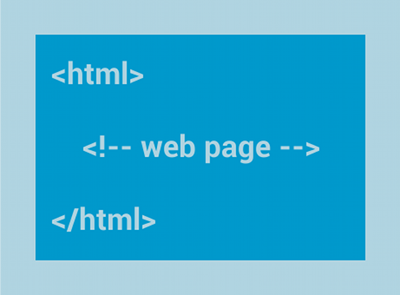
\includegraphics[width=\linewidth]{02-layouts/webview.png}
  \caption{Web View}
\endminipage
\end{figure}

\Subsection{Создание макета через Adapter}

Когда содержимое layout динамически изменяется или заранее не известно, можно
использовать layout, который является подклассом \AdapterView, чтобы заполнять
layout различными \View во время выполнения. Подклассы класса \AdapterView
используют \Adapter, чтобы привязать данные к layout. \Adapter выступает в роли
посредника между источником данных и \AdapterView -- \Adapter получает данные
(из таких источников как массив или база данных) и конвертирует каждую запись
во \View, который может быть добавлен в layout \AdapterView.

Некоторые типичные layout, которые создаются с помощью \Adapter:
\begin{itemize}
  \item \textbf{List View}. Отображает прокручиваемую колонку.
  
  \item \textbf{Grid View}. Отображает прокручиваемую таблицу.
\end{itemize}

\begin{figure}[H]
\centering
\minipage{0.25\textwidth}
  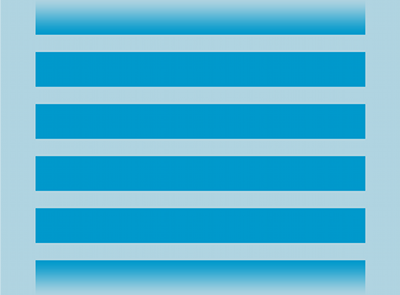
\includegraphics[width=\linewidth]{02-layouts/listview.png}
  \caption{List View}
\endminipage\hspace{1cm}
\minipage{0.25\textwidth}
  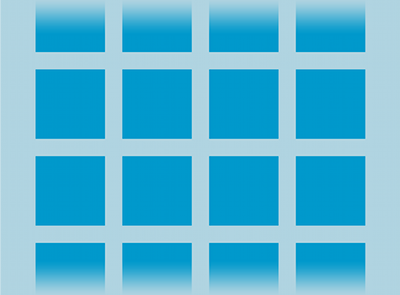
\includegraphics[width=\linewidth]{02-layouts/gridview.png}
  \caption{Grid View}
\endminipage
\end{figure}


